\hypertarget{threads-concurrency}{%
\section{Threads-Concurrency}\label{threads-concurrency}}

In den Folien steht nicht wirklich etwas sinnvolles\ldots{}

\subsection{Amdahls Law}
Das Gesetz von Amdahl besagt, wie viel von einem Programm paralellisiert werden kann.
\begin{figure}[H]
\centering
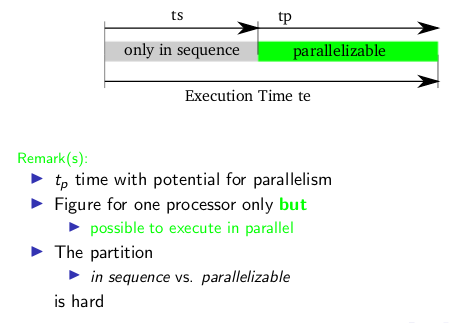
\includegraphics[width=0.6\textwidth]{figures/amdahl.png}
\caption{Amdahl}
\end{figure}

\clearpage